\documentclass[11pt,]{article}
\usepackage{lmodern}
\usepackage{amssymb,amsmath}
\usepackage{ifxetex,ifluatex}
\usepackage{fixltx2e} % provides \textsubscript
\ifnum 0\ifxetex 1\fi\ifluatex 1\fi=0 % if pdftex
  \usepackage[T1]{fontenc}
  \usepackage[utf8]{inputenc}
\else % if luatex or xelatex
  \ifxetex
    \usepackage{mathspec}
  \else
    \usepackage{fontspec}
  \fi
  \defaultfontfeatures{Ligatures=TeX,Scale=MatchLowercase}
  \newcommand{\euro}{€}
\fi
% use upquote if available, for straight quotes in verbatim environments
\IfFileExists{upquote.sty}{\usepackage{upquote}}{}
% use microtype if available
\IfFileExists{microtype.sty}{%
\usepackage{microtype}
\UseMicrotypeSet[protrusion]{basicmath} % disable protrusion for tt fonts
}{}
\usepackage[margin=1.0in]{geometry}
\usepackage{hyperref}
\PassOptionsToPackage{usenames,dvipsnames}{color} % color is loaded by hyperref
\hypersetup{unicode=true,
            pdftitle={OptiClust: Improved method for assigning amplicon-based sequence data to operational taxonomic units},
            pdfborder={0 0 0},
            breaklinks=true}
\urlstyle{same}  % don't use monospace font for urls
\usepackage{longtable,booktabs}
\usepackage{graphicx,grffile}
\makeatletter
\def\maxwidth{\ifdim\Gin@nat@width>\linewidth\linewidth\else\Gin@nat@width\fi}
\def\maxheight{\ifdim\Gin@nat@height>\textheight\textheight\else\Gin@nat@height\fi}
\makeatother
% Scale images if necessary, so that they will not overflow the page
% margins by default, and it is still possible to overwrite the defaults
% using explicit options in \includegraphics[width, height, ...]{}
\setkeys{Gin}{width=\maxwidth,height=\maxheight,keepaspectratio}
\setlength{\parindent}{0pt}
\setlength{\parskip}{6pt plus 2pt minus 1pt}
\setlength{\emergencystretch}{3em}  % prevent overfull lines
\providecommand{\tightlist}{%
  \setlength{\itemsep}{0pt}\setlength{\parskip}{0pt}}
\setcounter{secnumdepth}{0}

%%% Use protect on footnotes to avoid problems with footnotes in titles
\let\rmarkdownfootnote\footnote%
\def\footnote{\protect\rmarkdownfootnote}

%%% Change title format to be more compact
\usepackage{titling}

% Create subtitle command for use in maketitle
\newcommand{\subtitle}[1]{
  \posttitle{
    \begin{center}\large#1\end{center}
    }
}

\setlength{\droptitle}{-2em}
  \title{\textbf{OptiClust: Improved method for assigning amplicon-based sequence
data to operational taxonomic units}}
  \pretitle{\vspace{\droptitle}\centering\huge}
  \posttitle{\par}
  \author{}
  \preauthor{}\postauthor{}
  \date{}
  \predate{}\postdate{}


% Redefines (sub)paragraphs to behave more like sections
\ifx\paragraph\undefined\else
\let\oldparagraph\paragraph
\renewcommand{\paragraph}[1]{\oldparagraph{#1}\mbox{}}
\fi
\ifx\subparagraph\undefined\else
\let\oldsubparagraph\subparagraph
\renewcommand{\subparagraph}[1]{\oldsubparagraph{#1}\mbox{}}
\fi

\usepackage{helvet} % Helvetica font
\renewcommand*\familydefault{\sfdefault} % Use the sans serif version of the font
\usepackage[T1]{fontenc}

\usepackage[none]{hyphenat}

\usepackage{setspace}
\doublespacing
\setlength{\parskip}{1em}

\usepackage{lineno}

\usepackage{pdfpages}
\usepackage{comment}




\usepackage{multirow}
\usepackage{array}
\newcommand{\bigcell}[2]{\begin{tabular}{@{}#1@{}}#2\end{tabular}}
\usepackage{caption}

\begin{document}
\maketitle

\begin{center}

Running title: OptiClust: Optimized Clustering


\vspace{25mm}
Sarah L. Westcott and Patrick D. Schloss${^\dagger}$

\vspace{30mm}

$\dagger$ To whom correspondence should be addressed: pschloss@umich.edu

Department of Microbiology and Immunology, University of Michigan, Ann Arbor, MI
\end{center}

\newpage

\linenumbers

\subsection{Abstract}\label{abstract}

Assignment of 16S rRNA gene sequences to operational taxonomic units
(OTUs) is a computational bottleneck in the process of analyzing
microbial communities. Although this has been an active area of
research, it has been difficult to overcome the time and memory demands
while improving the quality of the OTU assignments. Here we developed a
new OTU assignment algorithm that iteratively reassigns sequences to new
OTUs to optimize the Matthews correlation coefficient (MCC), a measure
of the quality of OTU assignments. To assess the new algorithm,
OptiClust, we compared it to ten other algorithms using 16S rRNA gene
sequences from two simulated and four natural communities. Using the
OptiClust algorithm, the MCC values averaged 15.2 and 16.5\% higher than
the OTUs generated when we used the average neighbor and distance-based
greedy clustering with VSEARCH, respectively. Furthermore, on average,
OptiClust was 94.6-times faster than the average neighbor algorithm and
just as fast as distance-based greedy clustering with VSEARCH. An
empirical analysis of the efficiency of the algorithms showed that the
time and memory required to perform the algorithm scaled quadratically
with the number of unique sequences in the dataset. The significant
improvement in the quality of the OTU assignments over previously
existing methods will significantly enhance downstream analysis by
limiting the splitting of similar sequences into separate OTUs and
merging of dissimilar sequences into the same OTU. The development of
the OptiClust algorithm represents a significant advance that is likely
to have numerous other applications.

\subsection{Importance}\label{importance}

The analysis of microbial communities from diverse environments using
16S rRNA gene sequencing has expanded our knowledge of the biogeography
of microorganisms. An important step in this analysis is the assignment
of sequences into taxonomic groups based on their similarity to
sequences in a database or based on their similarity to each other,
irrespective of a database. In this study, we present a new algorithm
for the latter approach. The algorithm, OptiClust, seeks to optimize a
metric of assignment quality by shuffling sequences between taxonomic
groups. We found that OptiClust produces more robust assignments and
does so in a rapid and memory efficient manner. This advance will allow
for a more robust analysis of microbial communities and the factors that
shape them.

\newpage

\subsection{Introduction}\label{introduction}

Amplicon-based sequencing has provided incredible insights into Earth's
microbial biodiversity (1, 2). It has become common for studies to
include sequencing millions of 16S rRNA gene sequences across hundreds
of samples (3, 4). This is three to four orders of magnitude greater
sequencing depth than was previously achieved using Sanger sequencing
(5, 6). The increased sequencing depth has revealed novel taxonomic
diversity that is not adequately represented in reference databases (1,
3). However, the advance has forced re-engineering of methods to
overcome the rate and memory limiting steps in computational pipelines
that process raw sequences through the generation of tables containing
the number of sequences in different taxa for each sample (7--10). A
critical component to these pipelines has been the assignment of
amplicon sequences to taxonomic units that are ether defined based on
similarity to a reference or operationally based on the similarity of
the sequences to each other within the dataset (11, 12).

A growing number of algorithms have been developed to cluster sequences
into OTUs. These algorithms can be classified into three general
categories. The first category of algorithms has been termed
closed-reference or phylotyping (13, 14). Sequences are compared to a
reference collection and clustered based on the reference sequences that
they are similar to. This approach is fast; however, the method
struggles when a sequence is similar to multiple reference sequences
that may have different taxonomies and when it is not similar to
sequences in the reference. The second category of algorithms has been
called \emph{de novo} because they assign sequences to OTUs without the
use of a reference (14). These include hierarchical algorithms such as
nearest, furthest, and average neighbor (15) and algorithms that employ
heuristics such as abundance or distance-based greedy clustering as
implemented in USEARCH (16) or VSEARCH (17), Sumaclust, OTUCLUST (18),
and Swarm (19). \emph{De novo} methods tend to be more computationally
intense and it has proven difficult to know which method generates the
best assignments. A third category of algorithm is open-reference
clustering, which is a hybrid approach (3, 14). Here sequences are
assigned to OTUs using closed-reference clustering and sequences that
are not within a threshold of a reference sequence are then clustered
using a \emph{de novo} approach. This category blends the strengths and
weaknesses of the other method and adds the complication that
closed-reference and \emph{de novo} clustering use different OTU
definitions. These algorithms take different approaches to handling
large datasets to minimize the time and memory requirements while
attempting to assign sequences to meaningful OTUs.

Several metrics have emerged for assessing the quality of OTU assignment
algorithms. These have included the time and memory required to run the
algorithm (3, 19--21), agreement between OTU assignments and the
sequences' taxonomy (19, 21--31), sensitivity of an algorithm to
stochastic processes (32), the number of OTUs generated by the algorithm
(22, 33), and the ability to regenerate the assignments made by other
algorithms (3, 34). Unfortunately, these methods fail to directly
quantify the quality of the OTU assignments. An algorithm may complete
with minimal time and memory requirements or generate an idealized
number of OTUs, but the composition of the OTUs could be incorrect.
These metrics also tend to be subjective. For instance, a method may
appear to be recapitulate the taxonomy of a synthetic community with
known taxonomic structure, but do a poor job when applied to real
communities with poorly defined taxonomic structure or for sequences
that are prone to misclassification. As an alternative, we developed an
approach to objectively benchmark the clustering quality of OTU
assignments (13, 35, 36). This approach counts the number of true
positives (TP), true negatives (TN), false positives (FP), and false
negatives (FN) based on the pairwise distances. Sequence pairs that are
within the user-specified threshold and are clustered together represent
TPs and those in different OTUs are FNs. Those sequence pairs that have
a distance larger than the threshold and are not clustered in the same
OTU are TNs and those in the same OTU are FPs. These values can be
synthesized into a single correlation coefficient, the Matthews'
Correlation Coefficient (MCC), which measures the correlation between
observed and predicted classifications and is robust to cases where
there is an uneven distribution across the confusion matrix (37).
Consistently, the average neighbor algorithm was identified as among the
best or the best algorithm. The distance-based greedy clustering as
implemented in VSEARCH has also performed well. The computational
resources required to complete the average neighbor algorithm can be
significant for large datasets and so there is a need for an algorithm
that efficiently produces consistently high quality OTU assignments.

These previous efforts have assessed the quality of the clusters after
the completion of the algorithm. In the current study we developed and
benchmarked a new \emph{de novo} clustering algorithm that uses real
time calculation of the MCC to direct the progress of the clustering.
The result is the OptiClust algorithm, which produces significantly
better sequence assignments while making efficient use of computational
resources.

\subsection{Results}\label{results}

\textbf{\emph{OptiClust algorithm.}} The OptiClust algorithm uses the
pairs of sequences that are within a desired threshold of each other
(e.g.~0.03), a list of all sequence names in the dataset, and the metric
that should be used to assess clustering quality. A detailed description
of the algorithm is provided for a toy dataset in the Supplementary
Material. Briefly, the algorithm starts by placing each sequence either
within its own OTU or into a single OTU. The algorithm proceeds by
interrogating each sequence and re-calculating the metric for the cases
where the sequence stays in its current OTU, is moved to each of the
other OTUs, or is moved into a new OTU. The location that results in the
best clustering quality indicates whether the sequence should remain in
its current OTU or be moved to a different or new OTU. Each iteration
consists of interrogating every sequence in the dataset. Although
numerous options are available within the mothur-based implementation of
the algorithm (e.g.~sensitivity, specificity, accuracy, F1 score, etc.),
the default metric is MCC because it includes all four parameters from
the confusion matrix. The algorithm continues until the optimization
metric stabilizes or until it reaches a defined stopping criteria.

\textbf{\emph{OptiClust-generated OTUs are more robust than those from
other methods.}} To evaluate the OptiClust algorithm and compare its
performance to other algorithms, we utilized six datasets including two
synthetic communities and four previously published large datasets
generated from soil, marine, human, and murine samples (Table 1). When
we seeded the OptiClust algorithm with each sequence in a separate OTU
and ran the algorithm until complete convergence, the MCC values
averaged 15.2 and 16.5\% higher than the OTUs using average neighbor and
distance-based greedy clustering (DGC) with VSEARCH, respectively
(Figure 1). The number of OTUs formed by the various methods was
negatively correlated with their MCC value (\(\rho\)=-0.47; p=0). The
OptiClust algorithm was considerably faster than the hierarchical
algorithms and somewhat slower than the heuristic-based algorithms.
Across the six datasets, the OptiClust algorithm was 94.6-times faster
than average neighbor and just as fast as DGC with VSEARCH. The human
dataset was a challenge for a number of the algorithms. OTUCLUST and
SumaClust were unable to cluster the human dataset in less than 50 hours
and the average neighbor algorithm required more than 45 GB of RAM. The
USEARCH-based methods were unable to cluster the human data using the
32-bit free version of the software that limits the amount of RAM to
approximately 3.5 GB. These data demonstrate that OptiClust generated
significantly more robust OTU assignments than existing methods across a
diverse collection of datasets with performance that was comparable to
popular methods.

\textbf{\emph{OptiClust stopping criteria.}} By default, the
mothur-based implementation of the algorithm stops when the optimization
metric changes by less than 0.0001; however, this can be altered by the
user. This implementation also allows the user to stop the algorithm if
a maximum number of iterations is exceeded. By default mothur uses a
maximum value of 100 iterations. The justification for allowing
incomplete convergence was based on the observation that numerous
iterations are performed that extend the time required to complete the
clustering with minimal improvement in clustering. We evaluated the
results of clustering to partial convergence (i.e.~a change in the MCC
value that was less than 0.0001) or until complete convergence of the
MCC value (i.e.~until it did not change between iterations) when seeding
the algorithm with each sequence in a separate OTU (Figure 1). The small
difference in MCC values between the output from partial and complete
convergence resulted in a difference in the median number of OTUs that
ranged between 1.5 and 17.0 OTUs. This represented a difference of less
than 0.15\%. Among the four natural datasets, between 3 and 6 were
needed to achieve partial convergence and between 8 and 12.50 iterations
were needed to reach full convergence. The additional steps required
between 1.4 and 1.7 times longer to complete the algorithm. These
results suggest that achieving full convergence of the optimization
metric adds computational effort; however, considering full convergence
took between 2 and 17 minutes the extra effort was relatively small.
Although the mothur's default setting is partial convergence, the
remainder of our analysis used complete convergence to be more
conservative.

\textbf{\emph{Effect of seeding OTUs on OptiClust performance.}} By
default the mothur implementation of the OptiClust algorithm starts with
each sequence in a separate OTU. An alternative approach is to start
with all of the sequences in a single OTU. We found that the MCC values
for clusters generated seeding OptiClust with the sequences as a single
OTU were between 0 and 11.5\% lower than when seeding the algorithm with
sequences in separate OTUs (Figure 1). Interestingly, with the exception
of the human dataset (0.2\% more OTUs), the number of OTUs was as much
as 7.0\% lower (mice) than when the algorithm was seeded with sequence
in separate OTUs. Finally, the amount of time required to cluster the
data when the algorithm was seeded with a single OTU was between 1.5 and
2.9-times longer than if sequences were seeded as separate OTUs. This
analysis demonstrates that seeding the algorithm with sequences as
separate OTUs resulted in the best OTU assignments in the shortest
amount of time.

\textbf{\emph{OptiClust-generated OTUs are as stable as those from other
algorithms.}} One concern that many have with \emph{de novo} clustering
algorithms is that their output is sensitive to the initial order of the
sequences. An additional concern with the OptiClust algorithm is that it
may stabilize at a local optimum. To evaluate these concerns we compared
the results obtained using ten randomizations of the order that
sequences were given to the algorithm. The median the coefficient of
variation across the six datasets for MCC values obtained from the
replicate clusterings using OptiClust was 0.1\% (Figure 1). We also
measured the coefficient of variation for the number of OTUs across the
six datasets for each method. The median coefficient of variation for
the number of OTUs generated using OptiClust was 0.1\%. Confirming our
previous results, all of the methods we tested were stable to stochastic
processes. Of the methods that involved randomization, the coefficient
of variation for MCC values considerably smaller with OptiClust than the
other methods and the coefficient of variation for the number of OTUs
was comparable to the other methods. The variation observed in
clustering quality suggested that the algorithm does not appear to
converge to a locally optimum MCC value. More importantly, the random
variation does yield output of a similarly high quality.

\textbf{\emph{Time and memory required to complete Optimization-based
clustering scales efficiently.}} Although not as important as the
quality of clustering, the amount of time and memory required to assign
sequences to OTUs is a legitimate concern. To evaluate how the speed and
memory usage scaled with the number of sequences in the dataset, we
measured the time required and maximum RAM usage to cluster 20, 40, 60,
80, and 100\% of the unique sequences from each of the natural datasets
using the OptiClust algorithm (Figure 2). Within each iteration of the
algorithm, each sequence is compared to every other sequence and each
comparison requires a recalculation of the confusion matrix. This would
result in a worst case algorithmic complexity on the order of N\^{}3,
where N is the number of unique sequences. Because the algorithm only
needs to keep track of the sequence pairs that are within the threshold
of each other, it is likely that the implementation of the algorithm is
more efficient. To empirically determine the algorithmic complexity, we
fit a power law function to the data in Figure 2A. We observed power
coefficients between 1.7 and 2.5 for the marine and human datasets,
respectively. The algorithm requires storing a matrix that contains the
pairs of sequences that are close to each other as well as a matrix that
indicates which sequences are clustered together. The memory required to
store these matrices is on the order of N\^{}2, where N is the number of
unique sequences. In fact, when we fit a power law function to the data
in Figure 2B, the power coefficients were 1.9. This analysis suggests
that doubling the number of sequences in a dataset would increase the
time required to cluster the data by 4 to 8-fold and increase the RAM
required by 4-fold. It is possible that future improvements to the
implementation of the algorithm could improve this performance.

\textbf{\emph{Cluster splitting heuristic generates OTUs that are as
good as non-split approach.}} We previously described a heuristic to
accelerate OTU assignments where sequences were first classified to
taxonomic groups and within each taxon sequences were assigned to OTUs
using the average neighbor clustering algorithm (13). This accelerated
the clustering and reduce the memory requirements because the number of
unique sequences is effectively reduced by splitting sequences across
taxonomic groups. Furthermore, because sequences in different taxonomic
groups are assumed to belong to different OTUs they are independent,
which permits parallelization and additional reduction in computation
time. Reduction in clustering quality are encountered in this approach
if there are errors in classification or if two sequences within the
desired threshold belong to different taxonomic groups. It is expected
that these errors would increase as the taxonomic level goes from
kingdom to genus. To characterize the clustering quality, we calculated
the MCC values using OptiClust, average neighbor, and DGC with VSEARCH
when splitting at each taxonomic level (Figure 3). For each method, the
MCC values decreased as the taxonomic resolution increased; however, the
decrease in MCC as not as large as the difference between clustering
methods. As the resolution of the taxonomic levels increased, the
clustering quality remained high, relative to clusters formed from the
entire dataset (i.e.~kingdom-level). The MCC values when splitting the
datasets at the class and genus levels were within 98.0 and 93.0\%,
respectively, of the MCC values obtained from the entire dataset. These
decreases in MCC value resulted in the formation of as many as 4.7 and
22.5\% more OTUs, respectively, than were observed from the entire
dataset. For the datasets included in the current analysis, the use of
the cluster splitting heuristic was probably not worth the loss in
clustering quality. However, as datasets become larger, it may be
necessary to use the heuristic to clustering the data into OTUs.

\subsection{Discussion}\label{discussion}

Myriad methods have been proposed for assigning 16S rRNA gene sequences
to OTUs that each claim improved performance based on speed, memory
usage, representation of taxonomic information, and number of OTUs. Each
of these metrics is subjective and do not actually indicate the quality
of the clustering. This led us to propose using the MCC as a metric for
assessing the quality of clustering, post hoc. Here, we described a new
clustering method that seeks to optimize clustering based on an
objective criterion that measures clustering quality in real time. In
the OptiClust algorithm clustering is driven by optimizing a metric that
assesses whether any two sequences should be grouped into the same OTU.
The result is clusters that are significantly more robust and is
efficient in the time and memory required to cluster the sequences into
OTUs. This makes it more tractable to analyze large datasets without
sacrificing clustering quality as was previously necessary using
heuristic methods.

The cluster optimization procedure is dependent on the metric that is
chosen for optimization. We employed the MCC because it includes the
four values from a confusion matrix. Other algorithms such as the
furthest neighbor and nearest neighbor algorithms minimize the number of
FP and FN, respectively; however, these suffer because the number of FN
and FP are not controlled (13, 15). Alternatively, one could optimize
based on the sensitivity, specificity, or accuracy, which are each based
on two values from the confusion matrix or they could optimize based on
the F1 score, which is based on three values from the confusion matrix.
Because these metrics do not balance all four parameters equally, it is
likely that one parameter will dominate in the optimization procedure.
For example, optimizing for sensitivity could lead to a large number of
FPs. Since we would like to minimize both FPs and FNs and not just the
total number of false assignments, we decided to optimize utilizing the
MCC. It is possible that other metrics could be developed and employed
for optimization of the clustering.

The OptiClust algorithm is relatively simple. For each sequence it
effectively ask whether the MCC value will increase if the sequence is
moved to a different OTU including creating a new OTU. If the value does
not change, it remains in the current OTU. The algorithm repeats until
the MCC value stabilizes. Assuming that the algorithm is seeded with
each sequence in a separate OTU, it does not appear that the algorithm
converges to a local optimum. Furthermore, execution of the algorithm
with different random number generator seeds produces OTU assignments of
consistently high quality. Future improvements to the implementation of
the algorithm could provide optimization to further improve its speed
and susceptibility to find a local optimum. Users are encourage to
repeat the OTU assignment several times to confirm that they have found
the best OTU assignments.

Our previous MCC-based analysis of clustering algorithms indicated that
the average neighbor algorithm consistently produced the best OTU
assignments with the DGC-based method using USEARCH also producing
robust OTU assignments. The challenge in using the average neighbor
algorithm is that it requires a large amount of RAM and is
computationally demanding. This led to the development of a splitting
approach that divides the clustering across distinct taxonomic groups
(13). The improved performance provided by the OptiClust algorithm
likely makes such splitting unnecessary for most current datasets. We
have demonstrated that although the OTU assignments made at the genus
level are still better than that of other methods, the quality is not as
good as that found without splitting. The loss of quality is likely due
to misclassification because of limitations in the clustering algorithms
and reference databases. The practical significance of such small
differences in clustering quality remain to be determined; however,
based on the current analysis, it does appear that the number of OTUs is
artificially inflated. Regardless, the best clustering quality should be
pursued given the available computer resources.

The time and memory required to execute the OptiClust algorithm scaled
proportionally to the number of unique sequences raised to the second
power. The power for the time requirement is affected by the similarity
of the sequences in the dataset with datasets containing more similar
sequences having a higher power. Also, the number of unique sequences is
the basis for both the amount of time and memory required to complete
the algorithm. Both the similarity of sequences and number of unique
sequences can be driven by the sequencing error since any errors will
increase the number of unique sequences and these sequences will be
closely related to the perfect sequence. This underscores the importance
of reducing the noise in the sequence data (7). If sequencing errors are
not remediated and are relatively randomly distributed, then it is
likely that the algorithm will require an unnecessary amount of time and
RAM to complete.

The rapid expansion in sequencing capacity has demanded that the
algorithms used to assign 16S rRNA gene sequences to OTUs be efficient
while maintaining robust assignments. Although database-based approaches
have been proposed to facilitate this analysis, they are limited by
their limited coverage of bacterial taxonomy and by the inconsistent
process used to name taxa. The ability to assign sequences to OTUs using
an algorithm that optimizes clustering by directly measuring quality
will significantly enhance downstream analysis. The development of the
OptiClust algorithm represents a significant advance that is likely to
have numerous other applications.

\subsection{Materials and Methods}\label{materials-and-methods}

\textbf{\emph{Sequence data and processing steps.}} To evaluate the
OptiClust and the other algorithms we created two synthetic sequence
collections and four sequence collections generated from previously
published studies. The V4 region of the 16S rRNA gene was used from all
datasets because it is a popular region that can be fully sequenced with
two-fold coverage using the commonly used MiSeq sequencer from Illumina
(7). The method for generating the simulated datasets followed the
approach used by Kopylova et al. (33) and Schloss (35). Briefly, we
randomly selected 10,000 uniques V4 fragments from 16S rRNA gene
sequences that were unique from the SILVA non-redundant database (38). A
community with an even relative abundance profile was generated by
specifying that each sequence had a frequency of 100 reads. A community
with a staggered relative abundance profile was generated by specifying
that the abundance of each sequence was a randomly drawn integer sampled
from a uniform distribution between 1 and 200. Sequence collections
collected from human feces (39), murine feces (40), soil (41), and
seawater (42) were used to characterize the algorithms' performance with
natural communities. These sequence collections were all generated using
paired 150 or 250 nt reads of the V4 region. We re-processed all of the
reads using a common analysis pipeline that included quality score-based
error correction (7), alignment against a SILVA reference database (38,
43), screening for chimeras using UCHIME (9), and classification using a
naive Bayesian classifier with the RDP training set requiring an 80\%
confidence score (10).

\textbf{\emph{Implementation of clustering algorithms.}} In addition to
the OptiClust algorithm we evaluated ten different \emph{de novo}
clustering algorithms. These included three hierarchical algorithms,
average neighbor, nearest neighbor, and furthest neighbor, which are
implemented in mothur (v.1.39.0) (11). Seven heuristic methods were also
used including abundance-based greedy clustering (AGC) and
(distance-based greedy clustering) DGC as implemented in USEARCH (v.6.1)
(16) and VSEARCH (v.2.3.3) ((17){]}, OTUCLUST (v.0.1) (18), SumaClust
(v.1.0.20), and Swarm (v.2.1.9) (19). With the exception of Swarm each
of these methods uses distance-based thresholds to report OTU
assignments.

\textbf{\emph{Benchmarking.}} We evaluated the quality of the sequence
clustering, reproducibility of the clustering, the speed of clustering,
and the amount of memory required to complete the clustering. To assess
the quality of the clusters generated by each method, we counted the
cells within a confusion matrix that indicated how well the clusterings
represented the distances between the pair of sequences (13). Pairs of
sequences that were in the same OTU and had a distance less than 3\%
were true positives (TPs), those that were in different OTUs and had a
distance greater than 3\% were true negatives (TNs), those that were in
the same OTU and had a distance greater than 3\% were false positives
(FPs), and those that were in different OTUs and had a distance less
than 3\% were false negatives (FNs). To synthesize the matrix into a
single metric we used the Matthews Correlation Coefficient using the
\texttt{sens.spec} command in mothur using the following equations.

\[
MCC = \frac{TP \times TN-FP \times FN}{\sqrt{(TP+FP)(TP+FN)(TN+FP)(TN+FN)} }
\]

To assess the reproducibility of the algorithms we randomized the
starting order of each sequence collection ten times and ran each
algorithm on each randomized collection. We then measured the MCC for
each randomization and quantified their percent coefficient of variation
(\% CV; 100 times the ratio of the standard deviation to the mean).

To assess how the the memory and time requirements scaled with the
number of sequences included in each sequence collection, we randomly
subsampled 20, 40, 60, or 80\% of the unique sequences in each
collection. We obtained 10 subsamples at each depth for each dataset and
ran each collection (N= 50 = 5 sequencing depths x 10 replicates)
through each of the algorithms. We used the timeout script to quantify
the maximum RAM used and the amount of time required to process each
sequence collection (\url{https://github.com/pshved/timeout}). We
limited each algorithm to 45 GB of RAM and 50 hours using a single
processor.

\textbf{\emph{Data and code availability.}} The workflow utilized
commands in GNU make (v.3.81), GNU bash (v.4.1.2), mothur (v.1.39.0)
(11), and R (v.3.3.2) (44). Within R we utilized the wesanderson
(v.0.3.2) (45), dplyr (v.0.5.0) (46), tidyr (v.0.6.0) (47), cowplot
(v.0.6.3) (48), and ggplot2 (v.2.2.0.9000) (49) packages. A reproducible
version of this manuscript and analysis is available at
\url{https://github.com/SchlossLab/Westcott_OptiClust_mSphere_2017}.

\subsection{Acknowledgements}\label{acknowledgements}

This work was supported through funding from the National Institutes of
Health to PDS (P30DK034933). SLW designed, implemented, and evaluated
the algorithm. PDS designed and evaluated the algorithm. Both authors
wrote and edited the manuscript.

\newpage

\textbf{Table 1. Description of datasets used to evaluate the OptiClust
algorithm and compare its performance to other algorithms.} Each dataset
contains sequences from the V4 region of the 16S rRNA gene. The even and
staggered datasets were generated by extracting the V4 region from full
length reference sequences and the datasets from the natural communities
were generated by sequencing the V4 region using a Illumina MiSeq with
either paired 150 or 250 nt reads.

\begin{longtable}[c]{@{}lcccc@{}}
\toprule
\textbf{Dataset (Ref.)} & \textbf{Read Length} & \textbf{Samples} &
\textbf{Total Seqs.} & \textbf{Unique Seqs.}\tabularnewline
\midrule
\endhead
Soil (41) & 150 & 18 & 948,243 & 143,677\tabularnewline
Marine (42) & 250 & 7 & 1,384,988 & 75,923\tabularnewline
Mice (40) & 250 & 360 & 2,825,495 & 32,447\tabularnewline
Human (39) & 250 & 489 & 20,951,841 & 121,281\tabularnewline
Even (33, 35) & NA & NA & 1,155,800 & 11,558\tabularnewline
Staggered (33, 35) & NA & NA & 1,156,550 & 11,558\tabularnewline
\bottomrule
\end{longtable}

\newpage

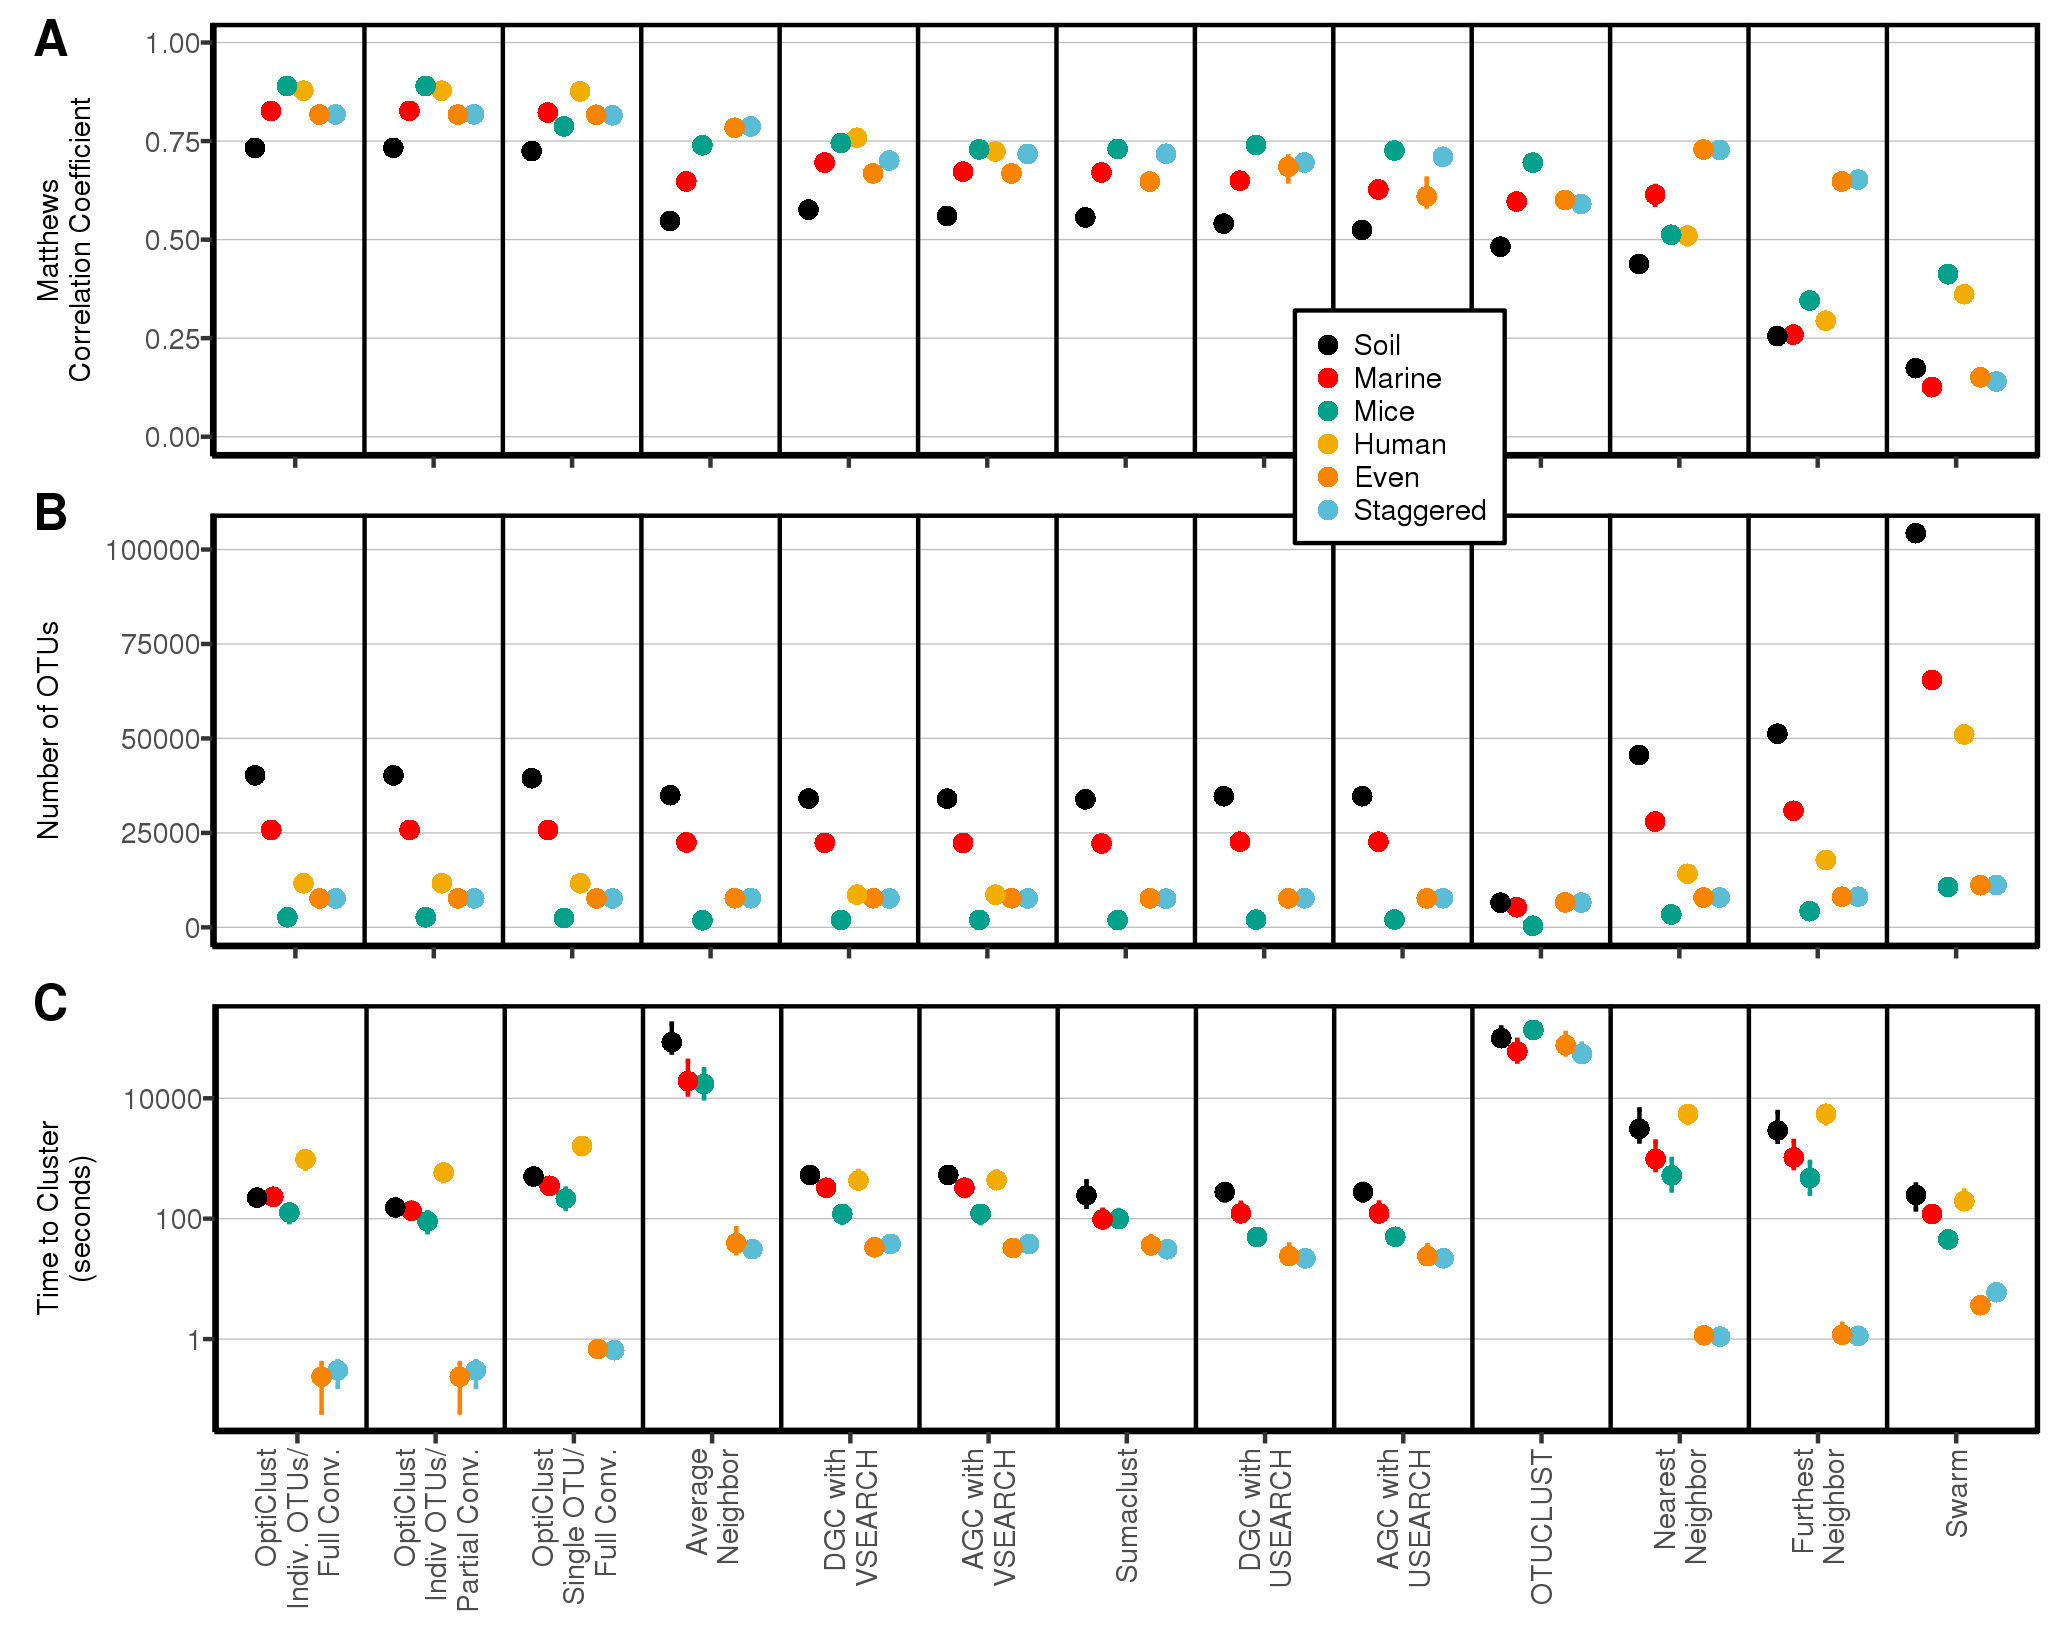
\includegraphics[width=6.0in]{../results/figures/performance.png}

\textbf{Figure 1. Comparison of de novo clustering algorithms.} Plot of
MCC (A), number of OTUs (B), and execution times (C) for the comparison
of \emph{de novo} clustering algorithms when applied to four natural and
two synthetic datasets. The first three columns of each figure contain
the results of clustering the datasets (i) seeding the algorithm with
one sequence per OTU and allowing the algorithm to proceed until the MCC
value no longer changed; (ii) seeding the algorithm with one sequence
per OTU and allowing the algorithm to proceed until the MCC changed by
less than 0.0001; (iii) seeding the algorithm with all of the sequences
in one OTU and allowing the algorithm to proceed until the MCC value no
longer changed. The human dataset could not be clustered by the average
neighbor, Sumaclust, USEARCH, or OTUCLUST with less than 45 GB of RAM or
50 hours of execution time. The median of 10 re-orderings of the data is
presented for each method and dataset. The range of observed values is
indicated by the error bars, which are typically smaller than the
plotting symbol.

\newpage

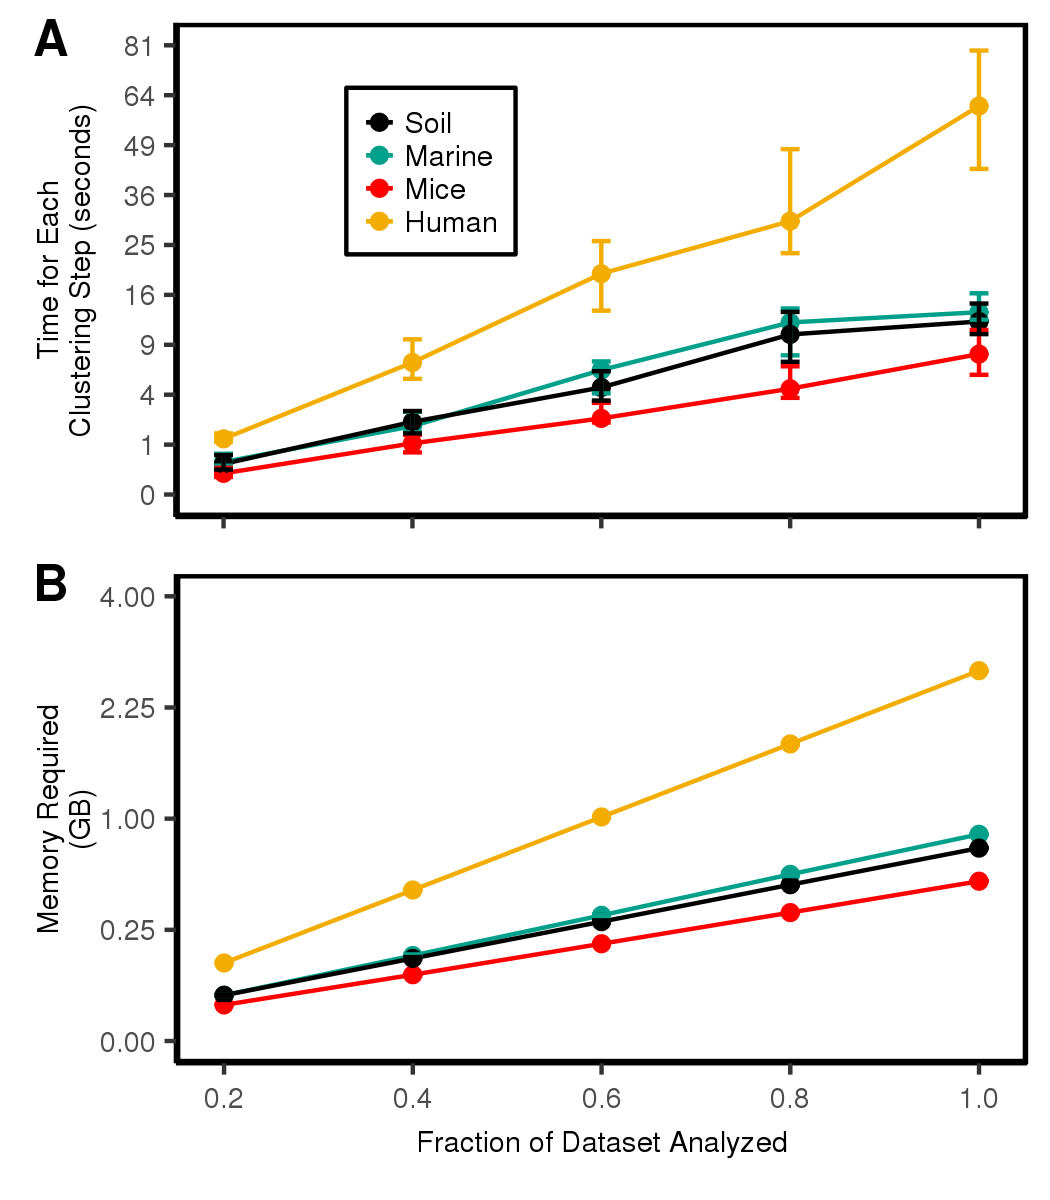
\includegraphics[width=3.5in]{../results/figures/speed_memory.png}

\textbf{Figure 2. OptiClust performance} The average execution time (A)
and memory usage (B) required to cluster the four natural datasets. The
confidence intervals indicate the range between the minimum and maximum
values. The y-axis is scaled by the square root to demonstrate the
relationship between the time and memory requirements relative to the
number of unique sequences squared.

\newpage

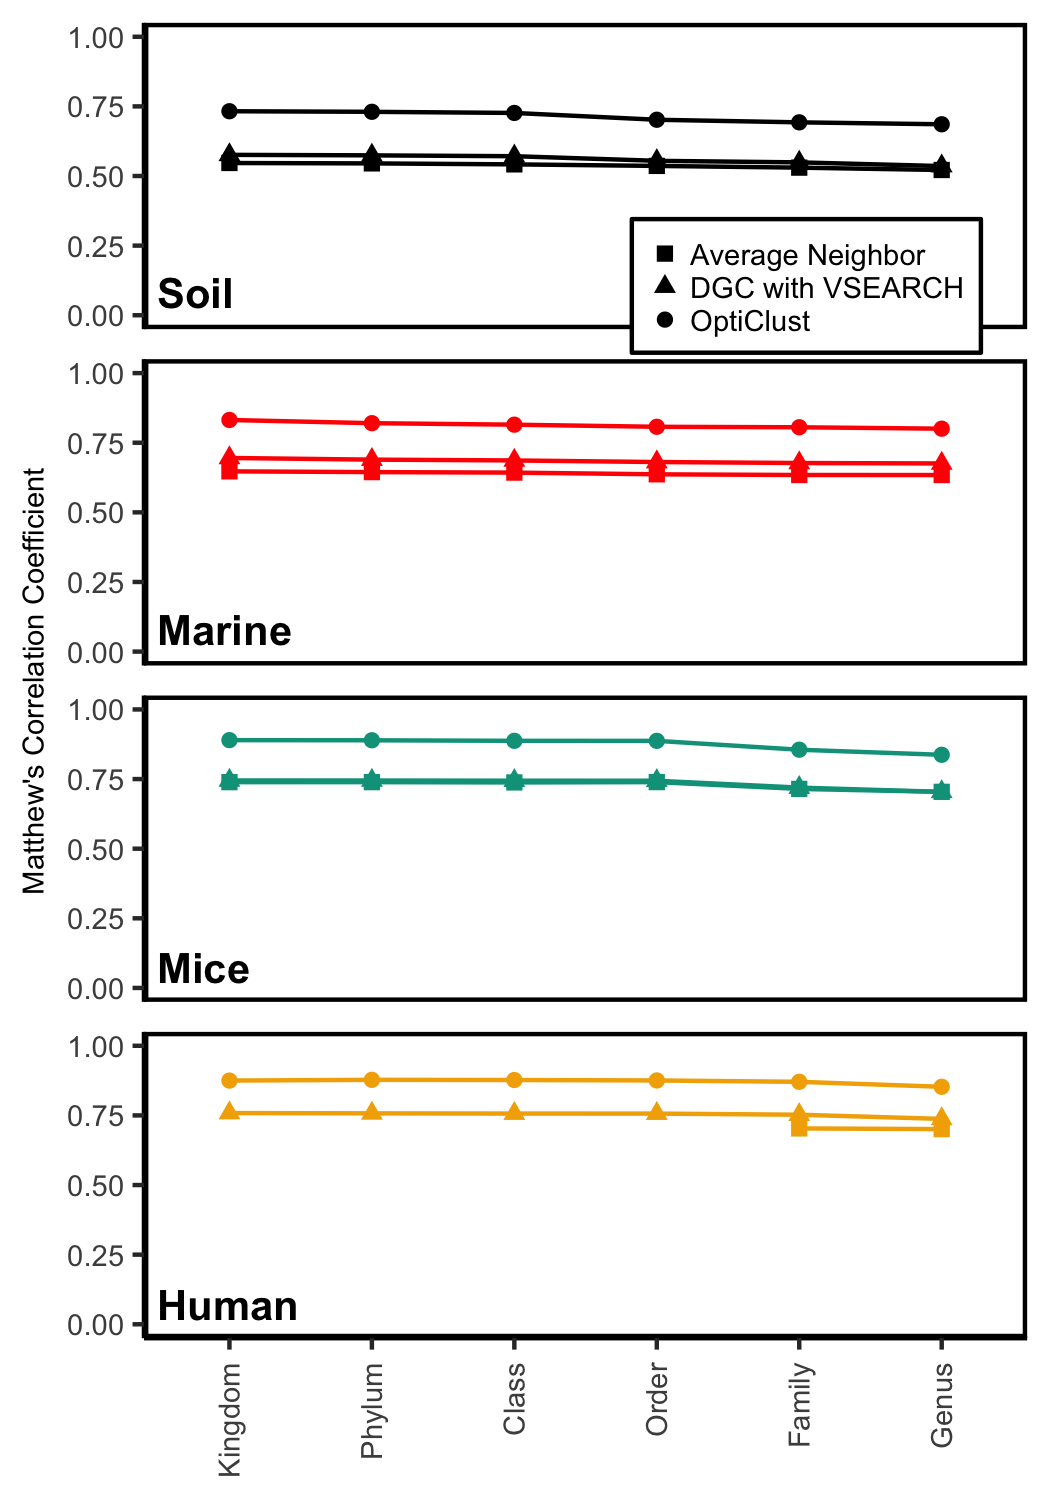
\includegraphics[width=3.5in]{../results/figures/split_mcc.png}

\textbf{Figure 3. Effects of taxonomically splitting the datasets on
clustering quality.} The datasets were split at each taxonomic level
based on their classification using a naive Bayesian classifier and
clustered using average neighbor, VSEARCH-based DGC, and OptiClust.

\newpage

\textbf{Supplemental text.} Worked example of how OptiClust algorithm
clusters sequences into OTUs.

\newpage

\subsection*{References}\label{references}
\addcontentsline{toc}{subsection}{References}

\hypertarget{refs}{}
\hypertarget{ref-Schloss2016b}{}
1. \textbf{Schloss PD}, \textbf{Girard RA}, \textbf{Martin T},
\textbf{Edwards J}, \textbf{Thrash JC}. 2016. Status of the archaeal and
bacterial census: An update. mBio \textbf{7}:e00201--16.
doi:\href{https://doi.org/10.1128/mbio.00201-16}{10.1128/mbio.00201-16}.

\hypertarget{ref-Locey2016}{}
2. \textbf{Locey KJ}, \textbf{Lennon JT}. 2016. Scaling laws predict
global microbial diversity. Proceedings of the National Academy of
Sciences \textbf{113}:5970--5975.
doi:\href{https://doi.org/10.1073/pnas.1521291113}{10.1073/pnas.1521291113}.

\hypertarget{ref-Rideout2014}{}
3. \textbf{Rideout JR}, \textbf{He Y}, \textbf{Navas-Molina JA},
\textbf{Walters WA}, \textbf{Ursell LK}, \textbf{Gibbons SM},
\textbf{Chase J}, \textbf{McDonald D}, \textbf{Gonzalez A},
\textbf{Robbins-Pianka A}, \textbf{Clemente JC}, \textbf{Gilbert JA},
\textbf{Huse SM}, \textbf{Zhou H-W}, \textbf{Knight R}, \textbf{Caporaso
JG}. 2014. Subsampled open-reference clustering creates consistent,
comprehensive OTU definitions and scales to billions of sequences. PeerJ
\textbf{2}:e545.
doi:\href{https://doi.org/10.7717/peerj.545}{10.7717/peerj.545}.

\hypertarget{ref-Huttenhower2012}{}
4. \textbf{Consortium THMP}. 2012. Structure, function and diversity of
the healthy human microbiome. Nature \textbf{486}:207--214.
doi:\href{https://doi.org/10.1038/nature11234}{10.1038/nature11234}.

\hypertarget{ref-Eckburg2005}{}
5. \textbf{Eckburg PB}, \textbf{Bik EM}, \textbf{Bernstein CN},
\textbf{Purdom E}, \textbf{Dethlefsen L}, \textbf{Sargent M},
\textbf{Gill SR}, \textbf{Nelson KE}, \textbf{Relman DA}. 2005.
Diversity of the human intestinal microbial flora. Science
\textbf{308}:1635--1638.

\hypertarget{ref-Elshahed2008}{}
6. \textbf{Elshahed MS}, \textbf{Youssef NH}, \textbf{Spain AM},
\textbf{Sheik C}, \textbf{Najar FZ}, \textbf{Sukharnikov LO},
\textbf{Roe BA}, \textbf{Davis JP}, \textbf{Schloss PD}, \textbf{Bailey
VL}, \textbf{Krumholz LR}. 2008. Novelty and uniqueness patterns of rare
members of the soil biosphere. Applied and Environmental Microbiology
\textbf{74}:5422--5428.
doi:\href{https://doi.org/10.1128/aem.00410-08}{10.1128/aem.00410-08}.

\hypertarget{ref-Kozich2013}{}
7. \textbf{Kozich JJ}, \textbf{Westcott SL}, \textbf{Baxter NT},
\textbf{Highlander SK}, \textbf{Schloss PD}. 2013. Development of a
dual-index sequencing strategy and curation pipeline for analyzing
amplicon sequence data on the MiSeq Illumina sequencing platform.
Applied and Environmental Microbiology \textbf{79}:5112--5120.
doi:\href{https://doi.org/10.1128/aem.01043-13}{10.1128/aem.01043-13}.

\hypertarget{ref-Schloss2009a}{}
8. \textbf{Schloss PD}. 2009. A high-throughput DNA sequence aligner for
microbial ecology studies. PLOS ONE \textbf{4}:e8230.
doi:\href{https://doi.org/10.1371/journal.pone.0008230}{10.1371/journal.pone.0008230}.

\hypertarget{ref-Edgar2011}{}
9. \textbf{Edgar RC}, \textbf{Haas BJ}, \textbf{Clemente JC},
\textbf{Quince C}, \textbf{Knight R}. 2011. UCHIME improves sensitivity
and speed of chimera detection. Bioinformatics \textbf{27}:2194--2200.
doi:\href{https://doi.org/10.1093/bioinformatics/btr381}{10.1093/bioinformatics/btr381}.

\hypertarget{ref-Wang2007}{}
10. \textbf{Wang Q}, \textbf{Garrity GM}, \textbf{Tiedje JM},
\textbf{Cole JR}. 2007. Naive bayesian classifier for rapid assignment
of rRNA sequences into the new bacterial taxonomy. Applied and
Environmental Microbiology \textbf{73}:5261--5267.
doi:\href{https://doi.org/10.1128/aem.00062-07}{10.1128/aem.00062-07}.

\hypertarget{ref-Schloss2009b}{}
11. \textbf{Schloss PD}, \textbf{Westcott SL}, \textbf{Ryabin T},
\textbf{Hall JR}, \textbf{Hartmann M}, \textbf{Hollister EB},
\textbf{Lesniewski RA}, \textbf{Oakley BB}, \textbf{Parks DH},
\textbf{Robinson CJ}, \textbf{Sahl JW}, \textbf{Stres B},
\textbf{Thallinger GG}, \textbf{Horn DJV}, \textbf{Weber CF}. 2009.
Introducing mothur: Open-source, platform-independent,
community-supported software for describing and comparing microbial
communities. Applied and Environmental Microbiology
\textbf{75}:7537--7541.
doi:\href{https://doi.org/10.1128/aem.01541-09}{10.1128/aem.01541-09}.

\hypertarget{ref-Caporaso2010}{}
12. \textbf{Caporaso JG}, \textbf{Kuczynski J}, \textbf{Stombaugh J},
\textbf{Bittinger K}, \textbf{Bushman FD}, \textbf{Costello EK},
\textbf{Fierer N}, \textbf{Peña AG}, \textbf{Goodrich JK},
\textbf{Gordon JI}, \textbf{Huttley GA}, \textbf{Kelley ST},
\textbf{Knights D}, \textbf{Koenig JE}, \textbf{Ley RE},
\textbf{Lozupone CA}, \textbf{McDonald D}, \textbf{Muegge BD},
\textbf{Pirrung M}, \textbf{Reeder J}, \textbf{Sevinsky JR},
\textbf{Turnbaugh PJ}, \textbf{Walters WA}, \textbf{Widmann J},
\textbf{Yatsunenko T}, \textbf{Zaneveld J}, \textbf{Knight R}. 2010.
QIIME allows analysis of high-throughput community sequencing data.
Nature Methods \textbf{7}:335--336.
doi:\href{https://doi.org/10.1038/nmeth.f.303}{10.1038/nmeth.f.303}.

\hypertarget{ref-Schloss2011}{}
13. \textbf{Schloss PD}, \textbf{Westcott SL}. 2011. Assessing and
improving methods used in operational taxonomic unit-based approaches
for 16S rRNA gene sequence analysis. Applied and Environmental
Microbiology \textbf{77}:3219--3226.
doi:\href{https://doi.org/10.1128/aem.02810-10}{10.1128/aem.02810-10}.

\hypertarget{ref-NavasMolina2013}{}
14. \textbf{Navas-Molina JA}, \textbf{Peralta-Sánchez JM},
\textbf{González A}, \textbf{McMurdie PJ}, \textbf{Vázquez-Baeza Y},
\textbf{Xu Z}, \textbf{Ursell LK}, \textbf{Lauber C}, \textbf{Zhou H},
\textbf{Song SJ}, \textbf{Huntley J}, \textbf{Ackermann GL},
\textbf{Berg-Lyons D}, \textbf{Holmes S}, \textbf{Caporaso JG},
\textbf{Knight R}. 2013. Advancing our understanding of the human
microbiome using QIIME, pp. 371--444. \emph{In} Methods in enzymology.
Elsevier BV.

\hypertarget{ref-Schloss2005}{}
15. \textbf{Schloss PD}, \textbf{Handelsman J}. 2005. Introducing DOTUR,
a computer program for defining operational taxonomic units and
estimating species richness. Applied and Environmental microbiology
\textbf{71}:1501--1506.

\hypertarget{ref-Edgar2010}{}
16. \textbf{Edgar RC}. 2010. Search and clustering orders of magnitude
faster than BLAST. Bioinformatics \textbf{26}:2460--2461.
doi:\href{https://doi.org/10.1093/bioinformatics/btq461}{10.1093/bioinformatics/btq461}.

\hypertarget{ref-Rognes2016}{}
17. \textbf{Rognes T}, \textbf{Flouri T}, \textbf{Nichols B},
\textbf{Quince C}, \textbf{Mahé F}. 2016. VSEARCH: A versatile open
source tool for metagenomics. PeerJ \textbf{4}:e2584.
doi:\href{https://doi.org/10.7717/peerj.2584}{10.7717/peerj.2584}.

\hypertarget{ref-Albanese2015}{}
18. \textbf{Albanese D}, \textbf{Fontana P}, \textbf{Filippo CD},
\textbf{Cavalieri D}, \textbf{Donati C}. 2015. MICCA: A complete and
accurate software for taxonomic profiling of metagenomic data.
Scientific Reports \textbf{5}:9743.
doi:\href{https://doi.org/10.1038/srep09743}{10.1038/srep09743}.

\hypertarget{ref-Mah2014}{}
19. \textbf{Mahé F}, \textbf{Rognes T}, \textbf{Quince C},
\textbf{Vargas C de}, \textbf{Dunthorn M}. 2014. Swarm: Robust and fast
clustering method for amplicon-based studies. PeerJ \textbf{2}:e593.
doi:\href{https://doi.org/10.7717/peerj.593}{10.7717/peerj.593}.

\hypertarget{ref-Sun2009}{}
20. \textbf{Sun Y}, \textbf{Cai Y}, \textbf{Liu L}, \textbf{Yu F},
\textbf{Farrell ML}, \textbf{McKendree W}, \textbf{Farmerie W}. 2009.
ESPRIT: Estimating species richness using large collections of 16S rRNA
pyrosequences. Nucleic Acids Research \textbf{37}:e76--e76.
doi:\href{https://doi.org/10.1093/nar/gkp285}{10.1093/nar/gkp285}.

\hypertarget{ref-Cai2011}{}
21. \textbf{Cai Y}, \textbf{Sun Y}. 2011. ESPRIT-tree: Hierarchical
clustering analysis of millions of 16S rRNA pyrosequences in quasilinear
computational time. Nucleic Acids Research \textbf{39}:e95--e95.
doi:\href{https://doi.org/10.1093/nar/gkr349}{10.1093/nar/gkr349}.

\hypertarget{ref-Edgar2013}{}
22. \textbf{Edgar RC}. 2013. UPARSE: Highly accurate OTU sequences from
microbial amplicon reads. Nature Methods \textbf{10}:996--998.
doi:\href{https://doi.org/10.1038/nmeth.2604}{10.1038/nmeth.2604}.

\hypertarget{ref-Mah2015}{}
23. \textbf{Mahé F}, \textbf{Rognes T}, \textbf{Quince C},
\textbf{Vargas C de}, \textbf{Dunthorn M}. 2015. Swarm v2:
Highly-scalable and high-resolution amplicon clustering. PeerJ
\textbf{3}:e1420.
doi:\href{https://doi.org/10.7717/peerj.1420}{10.7717/peerj.1420}.

\hypertarget{ref-Barriuso2011}{}
24. \textbf{Barriuso J}, \textbf{Valverde JR}, \textbf{Mellado RP}.
2011. Estimation of bacterial diversity using next generation sequencing
of 16S rDNA: A comparison of different workflows. BMC Bioinformatics
\textbf{12}:473.
doi:\href{https://doi.org/10.1186/1471-2105-12-473}{10.1186/1471-2105-12-473}.

\hypertarget{ref-Bonder2012}{}
25. \textbf{Bonder MJ}, \textbf{Abeln S}, \textbf{Zaura E},
\textbf{Brandt BW}. 2012. Comparing clustering and pre-processing in
taxonomy analysis. Bioinformatics \textbf{28}:2891--2897.
doi:\href{https://doi.org/10.1093/bioinformatics/bts552}{10.1093/bioinformatics/bts552}.

\hypertarget{ref-Chen2013}{}
26. \textbf{Chen W}, \textbf{Zhang CK}, \textbf{Cheng Y}, \textbf{Zhang
S}, \textbf{Zhao H}. 2013. A comparison of methods for clustering 16S
rRNA sequences into OTUs. PLOS ONE \textbf{8}:e70837.
doi:\href{https://doi.org/10.1371/journal.pone.0070837}{10.1371/journal.pone.0070837}.

\hypertarget{ref-Huse2010}{}
27. \textbf{Huse SM}, \textbf{Welch DM}, \textbf{Morrison HG},
\textbf{Sogin ML}. 2010. Ironing out the wrinkles in the rare biosphere
through improved OTU clustering. Environmental Microbiology
\textbf{12}:1889--1898.
doi:\href{https://doi.org/10.1111/j.1462-2920.2010.02193.x}{10.1111/j.1462-2920.2010.02193.x}.

\hypertarget{ref-May2014}{}
28. \textbf{May A}, \textbf{Abeln S}, \textbf{Crielaard W},
\textbf{Heringa J}, \textbf{Brandt BW}. 2014. Unraveling the outcome of
16S rDNA-based taxonomy analysis through mock data and simulations.
Bioinformatics \textbf{30}:1530--1538.
doi:\href{https://doi.org/10.1093/bioinformatics/btu085}{10.1093/bioinformatics/btu085}.

\hypertarget{ref-Sun2011}{}
29. \textbf{Sun Y}, \textbf{Cai Y}, \textbf{Huse SM}, \textbf{Knight R},
\textbf{Farmerie WG}, \textbf{Wang X}, \textbf{Mai V}. 2011. A
large-scale benchmark study of existing algorithms for
taxonomy-independent microbial community analysis. Briefings in
Bioinformatics \textbf{13}:107--121.
doi:\href{https://doi.org/10.1093/bib/bbr009}{10.1093/bib/bbr009}.

\hypertarget{ref-White2010}{}
30. \textbf{White JR}, \textbf{Navlakha S}, \textbf{Nagarajan N},
\textbf{Ghodsi M-R}, \textbf{Kingsford C}, \textbf{Pop M}. 2010.
Alignment and clustering of phylogenetic markers - implications for
microbial diversity studies. BMC Bioinformatics \textbf{11}:152.
doi:\href{https://doi.org/10.1186/1471-2105-11-152}{10.1186/1471-2105-11-152}.

\hypertarget{ref-AlGhalith2016}{}
31. \textbf{Al-Ghalith GA}, \textbf{Montassier E}, \textbf{Ward HN},
\textbf{Knights D}. 2016. NINJA-OPS: Fast accurate marker gene alignment
using concatenated ribosomes. PLOS Computational Biology
\textbf{12}:e1004658.
doi:\href{https://doi.org/10.1371/journal.pcbi.1004658}{10.1371/journal.pcbi.1004658}.

\hypertarget{ref-He2015}{}
32. \textbf{He Y}, \textbf{Caporaso JG}, \textbf{Jiang X-T},
\textbf{Sheng H-F}, \textbf{Huse SM}, \textbf{Rideout JR}, \textbf{Edgar
RC}, \textbf{Kopylova E}, \textbf{Walters WA}, \textbf{Knight R},
\textbf{Zhou H-W}. 2015. Stability of operational taxonomic units: An
important but neglected property for analyzing microbial diversity.
Microbiome \textbf{3}.
doi:\href{https://doi.org/10.1186/s40168-015-0081-x}{10.1186/s40168-015-0081-x}.

\hypertarget{ref-Kopylova2016}{}
33. \textbf{Kopylova E}, \textbf{Navas-Molina JA}, \textbf{Mercier C},
\textbf{Xu ZZ}, \textbf{Mahé F}, \textbf{He Y}, \textbf{Zhou H-W},
\textbf{Rognes T}, \textbf{Caporaso JG}, \textbf{Knight R}. 2016.
Open-source sequence clustering methods improve the state of the art.
mSystems \textbf{1}:e00003--15.
doi:\href{https://doi.org/10.1128/msystems.00003-15}{10.1128/msystems.00003-15}.

\hypertarget{ref-Schmidt2014}{}
34. \textbf{Schmidt TSB}, \textbf{Rodrigues JFM}, \textbf{Mering C von}.
2014. Limits to robustness and reproducibility in the demarcation of
operational taxonomic units. Environ Microbiol \textbf{17}:1689--1706.
doi:\href{https://doi.org/10.1111/1462-2920.12610}{10.1111/1462-2920.12610}.

\hypertarget{ref-Schloss2016a}{}
35. \textbf{Schloss PD}. 2016. Application of a database-independent
approach to assess the quality of operational taxonomic unit picking
methods. mSystems \textbf{1}:e00027--16.
doi:\href{https://doi.org/10.1128/msystems.00027-16}{10.1128/msystems.00027-16}.

\hypertarget{ref-Westcott2015}{}
36. \textbf{Westcott SL}, \textbf{Schloss PD}. 2015. De novo clustering
methods outperform reference-based methods for assigning 16S rRNA gene
sequences to operational taxonomic units. PeerJ \textbf{3}:e1487.
doi:\href{https://doi.org/10.7717/peerj.1487}{10.7717/peerj.1487}.

\hypertarget{ref-Matthews1975}{}
37. \textbf{Matthews B}. 1975. Comparison of the predicted and observed
secondary structure of t4 phage lysozyme. Biochimica et Biophysica Acta
(BBA) - Protein Structure \textbf{405}:442--451.
doi:\href{https://doi.org/10.1016/0005-2795(75)90109-9}{10.1016/0005-2795(75)90109-9}.

\hypertarget{ref-Pruesse2007}{}
38. \textbf{Pruesse E}, \textbf{Quast C}, \textbf{Knittel K},
\textbf{Fuchs BM}, \textbf{Ludwig W}, \textbf{Peplies J},
\textbf{Glockner FO}. 2007. SILVA: A comprehensive online resource for
quality checked and aligned ribosomal RNA sequence data compatible with
ARB. Nucleic Acids Research \textbf{35}:7188--7196.
doi:\href{https://doi.org/10.1093/nar/gkm864}{10.1093/nar/gkm864}.

\hypertarget{ref-Baxter2016}{}
39. \textbf{Baxter NT}, \textbf{Ruffin MT}, \textbf{Rogers MAM},
\textbf{Schloss PD}. 2016. Microbiota-based model improves the
sensitivity of fecal immunochemical test for detecting colonic lesions.
Genome Medicine \textbf{8}.
doi:\href{https://doi.org/10.1186/s13073-016-0290-3}{10.1186/s13073-016-0290-3}.

\hypertarget{ref-Schloss2012}{}
40. \textbf{Schloss PD}, \textbf{Schubert AM}, \textbf{Zackular JP},
\textbf{Iverson KD}, \textbf{Young VB}, \textbf{Petrosino JF}. 2012.
Stabilization of the murine gut microbiome following weaning. Gut
Microbes \textbf{3}:383--393.
doi:\href{https://doi.org/10.4161/gmic.21008}{10.4161/gmic.21008}.

\hypertarget{ref-Johnston2016}{}
41. \textbf{Johnston ER}, \textbf{Rodriguez-R LM}, \textbf{Luo C},
\textbf{Yuan MM}, \textbf{Wu L}, \textbf{He Z}, \textbf{Schuur EAG},
\textbf{Luo Y}, \textbf{Tiedje JM}, \textbf{Zhou J},
\textbf{Konstantinidis KT}. 2016. Metagenomics reveals pervasive
bacterial populations and reduced community diversity across the alaska
tundra ecosystem. Front Microbiol \textbf{7}.
doi:\href{https://doi.org/10.3389/fmicb.2016.00579}{10.3389/fmicb.2016.00579}.

\hypertarget{ref-Henson2016}{}
42. \textbf{Henson MW}, \textbf{Pitre DM}, \textbf{Weckhorst JL},
\textbf{Lanclos VC}, \textbf{Webber AT}, \textbf{Thrash JC}. 2016.
Artificial seawater media facilitate cultivating members of the
microbial majority from the gulf of mexico. mSphere
\textbf{1}:e00028--16.
doi:\href{https://doi.org/10.1128/msphere.00028-16}{10.1128/msphere.00028-16}.

\hypertarget{ref-Schloss2010}{}
43. \textbf{Schloss PD}. 2010. The effects of alignment quality,
distance calculation method, sequence filtering, and region on the
analysis of 16S rRNA gene-based studies. PLOS Comput Biol
\textbf{6}:e1000844.
doi:\href{https://doi.org/10.1371/journal.pcbi.1000844}{10.1371/journal.pcbi.1000844}.

\hypertarget{ref-language2015}{}
44. \textbf{R Core Team}. 2015. R: A language and environment for
statistical computing. R Foundation for Statistical Computing, Vienna,
Austria.

\hypertarget{ref-wesanderson}{}
45. \textbf{Ram K}, \textbf{Wickham H}. 2015. wesanderson: A wes
anderson palette generator.

\hypertarget{ref-dplyr}{}
46. \textbf{Wickham H}, \textbf{Francois R}. 2016. dplyr: A grammar of
data manipulation.

\hypertarget{ref-tidyr}{}
47. \textbf{Wickham H}. 2016. tidyr: Easily tidy data with `spread()`
and `gather()` functions.

\hypertarget{ref-cowplot}{}
48. \textbf{Wilke CO}. cowplot: Streamlined plot theme and plot
annotations for 'ggplot2'.

\hypertarget{ref-ggplot2}{}
49. \textbf{Wickham H}. 2009. ggplot2: Elegant graphics for data
analysis. Springer-Verlag New York.

\end{document}
